\documentclass[12pt]{article}

\usepackage[margin=1in]{geometry}
\usepackage[utf8]{inputenc}
\usepackage{multirow}
\usepackage{booktabs}
\usepackage{amsmath}
\usepackage{verbatim}
\usepackage{setspace}
\onehalfspacing
\usepackage{graphicx}
\graphicspath{{../Output/Figures/}}
\usepackage{tabularx}
\usepackage{indentfirst}
\usepackage[titletoc,title]{appendix}
\usepackage{subfigure}
%\usepackage{apacite}
\usepackage{natbib}
\setcitestyle{aysep={}}	
\usepackage{color}
\usepackage{longtable}
\usepackage{lscape}
\usepackage{pdflscape}
%\usepackage{subcaption}
\newcommand{\annote}[1]{\parbox{\textwidth}{\renewcommand{\baselinestretch}{1.0}\vspace{12pt} \small Notes: #1}}
\renewcommand{\vec}[1]{\mathbf{#1}}
\usepackage[usenames,dvipsnames,svgnames,table]{xcolor}
\usepackage{libertine}
\usepackage{hyperref}
\hypersetup{
     colorlinks   = true,
     citecolor    = black,
     linkcolor = black
}

\title{Adopting the Euro: a Synthetic Control Approach \\ Online Appendix\\ \vspace{2em}}

\date{\vspace{3em} January, 2024}

\author{\hspace{-2em} Ricardo Duque Gabriel\footnote{Corresponding author: Federal Reserve Board. E-mail address: ricardofilipeduquegabriel@gmail.com} \hspace{5em} Ana Sofia Pessoa\footnote{University of Bonn. E-mail address: sofiamendespessoa@gmail.com}\\ \hspace{-3em} University of Bonn and NBER \hspace{3em} University of Bonn}

\begin{document}
\begin{titlepage}
\clearpage\thispagestyle{empty}
\maketitle

\end{titlepage}

\section{Further Robustness Checks and Other Exercises}

\section{\label{SS_Components} Components Analysis}

\begin{figure}[h!]
    \centering
    \caption{\label{F_Components_AUT} Components of Austria's GDP}
    \subfigure[Private Consumption]{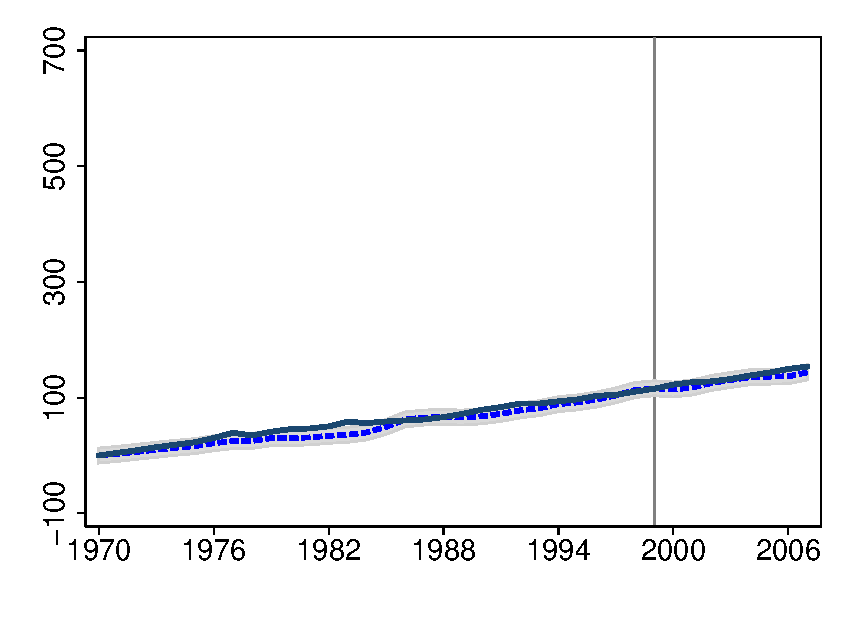
\includegraphics[width=8cm]{Composition/SCM_csh_c_1_Annual.eps}}
    \subfigure[Government Consumption]{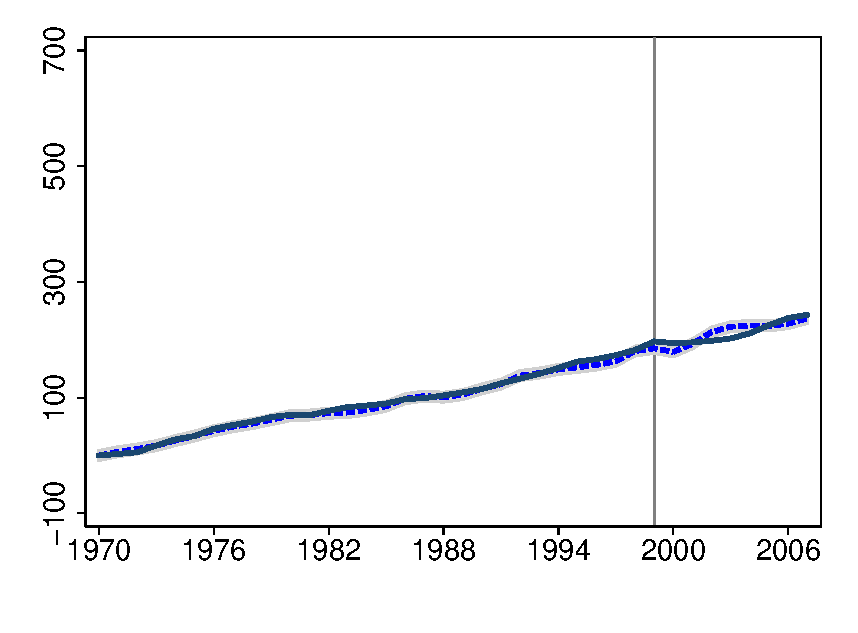
\includegraphics[width=8cm]{Composition/SCM_csh_g_1_Annual.eps}}
    \subfigure[Investment]{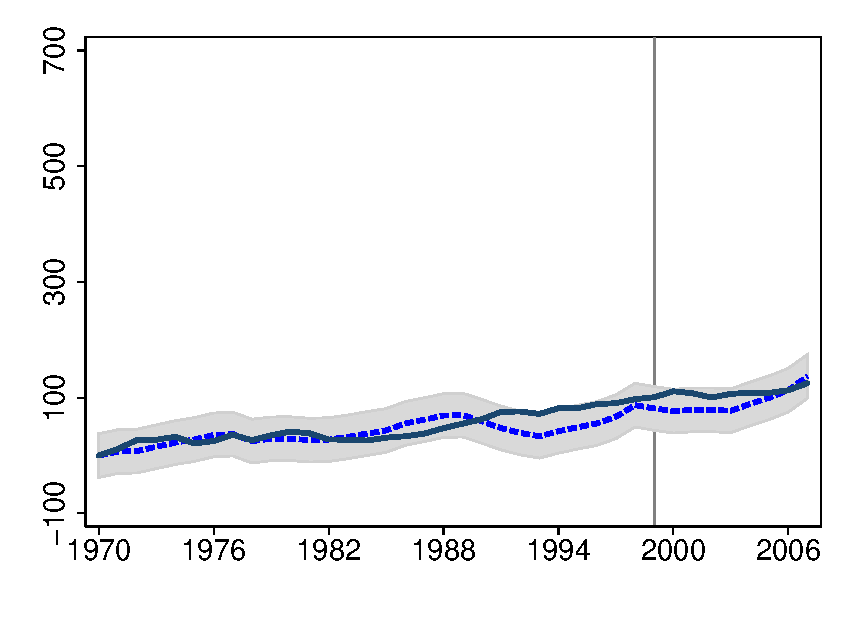
\includegraphics[width=8cm]{Composition/SCM_csh_i_1_Annual.eps}}
    \subfigure[Exports]{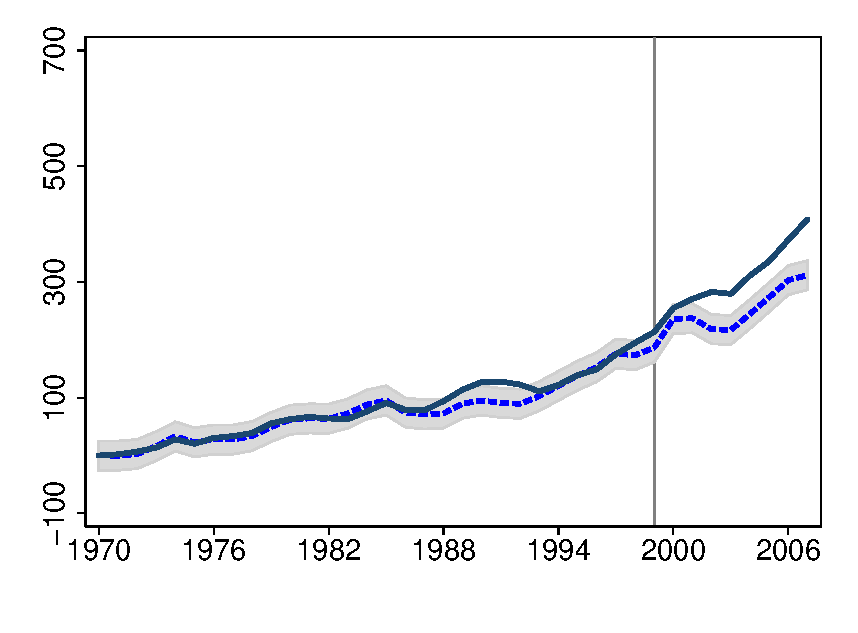
\includegraphics[width=8cm]{Composition/SCM_csh_x_1_Annual.eps}}
    \subfigure[Imports]{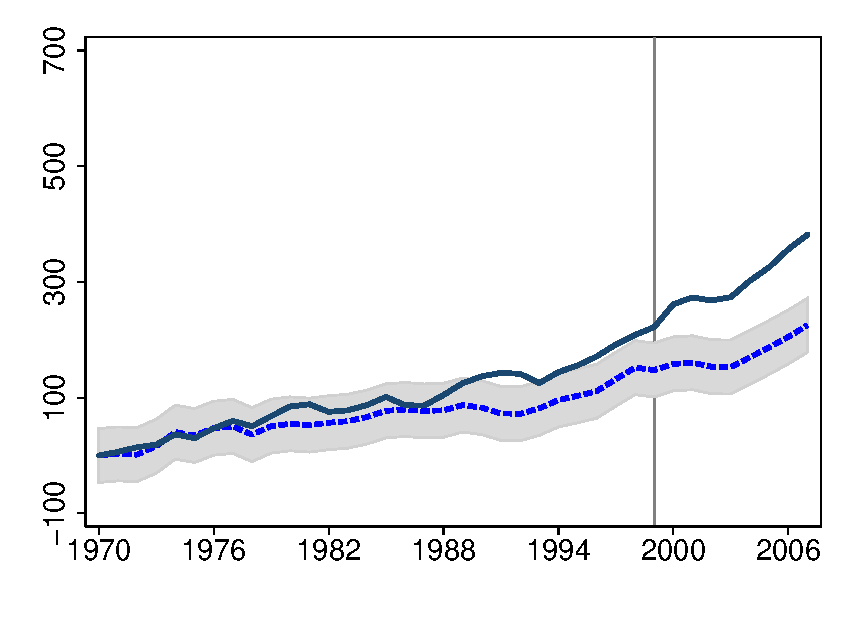
\includegraphics[width=8cm]{Composition/SCM_csh_m_1_Annual.eps}}
    \subfigure[Net Exports]{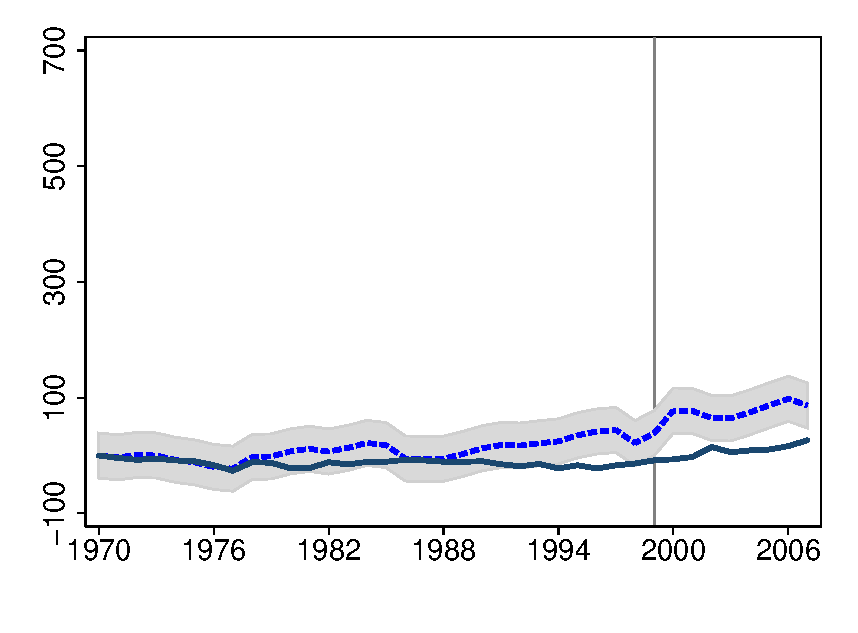
\includegraphics[width=8cm]{Composition/SCM_csh_nx_1_Annual.eps}}
    \annote{The plots depict, for each GDP component, the deviation in percent from the value of 1970. The blue dashed lines represents the synthetic Austria computed in section \ref{S_Doppelganger}. The full black lines stand for the actual Austrian series. The shaded area corresponds to two standard deviations of the difference between the treated country and the doppelganger prior to the euro accession.}
\end{figure}

\begin{figure}[h!]
    \centering
    \caption{\label{F_Components_BEL} Components of Belgium's GDP}
    \subfigure[Private Consumption]{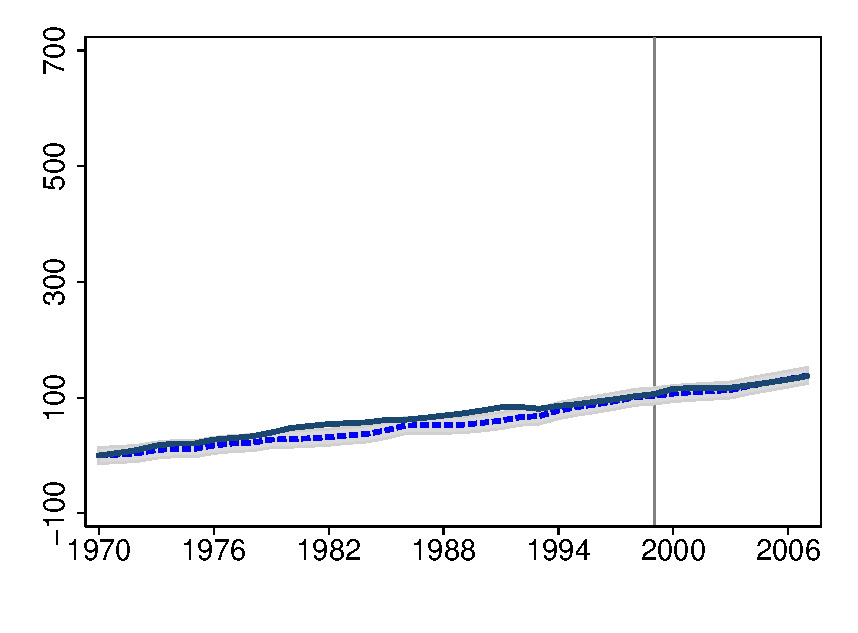
\includegraphics[width=8cm]{Composition/SCM_csh_c_3_Annual.eps}}
    \subfigure[Government Consumption]{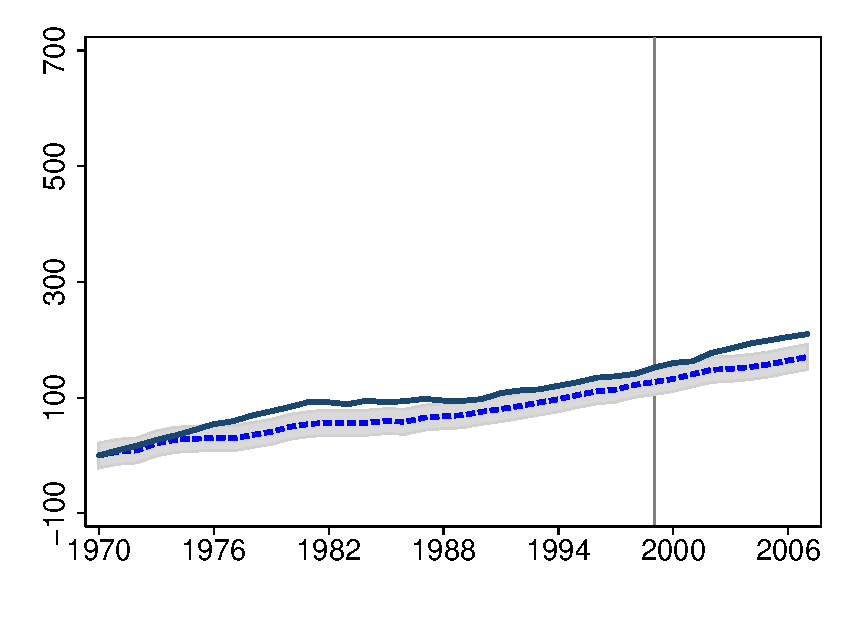
\includegraphics[width=8cm]{Composition/SCM_csh_g_3_Annual.eps}}
    \subfigure[Investment]{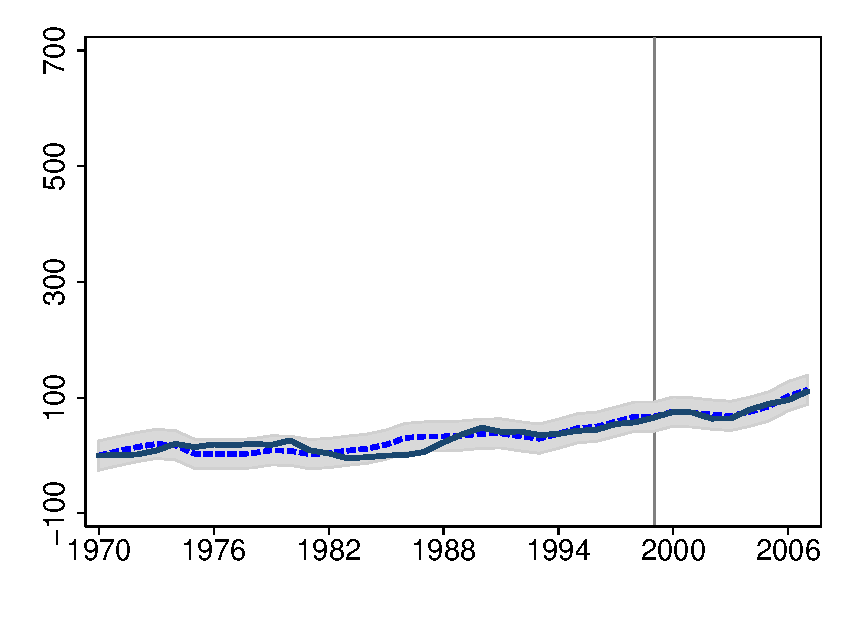
\includegraphics[width=8cm]{Composition/SCM_csh_i_3_Annual.eps}}
    \subfigure[Exports]{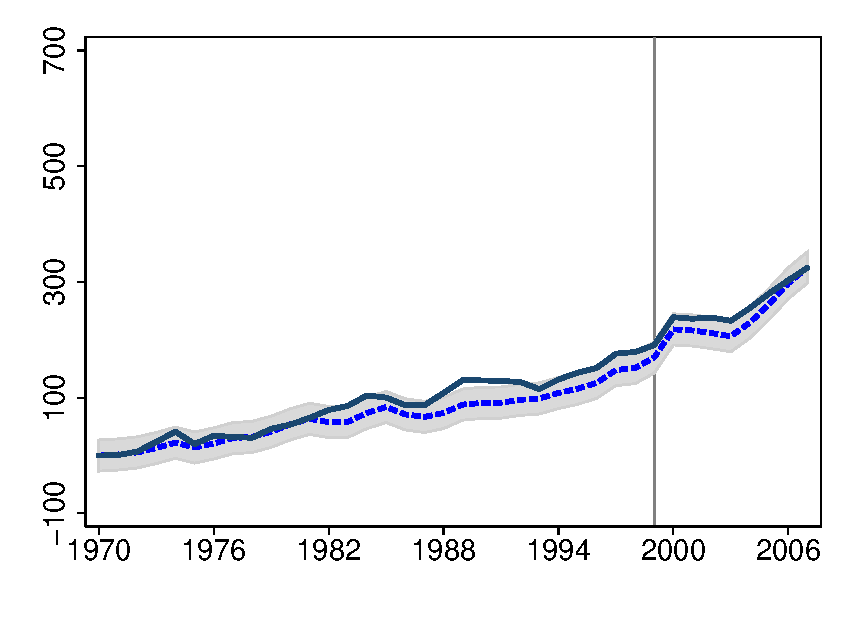
\includegraphics[width=8cm]{Composition/SCM_csh_x_3_Annual.eps}}
    \subfigure[Imports]{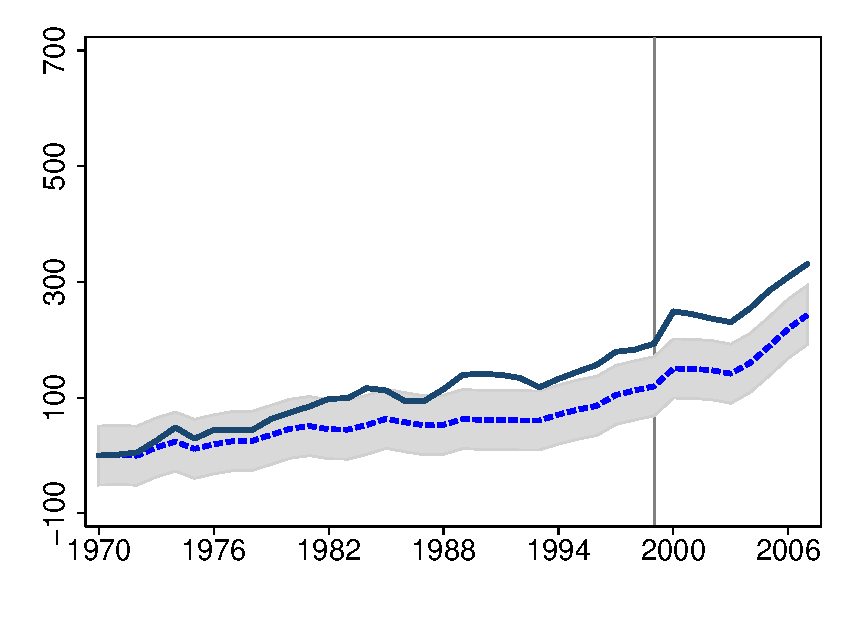
\includegraphics[width=8cm]{Composition/SCM_csh_m_3_Annual.eps}}
    \subfigure[Net Exports]{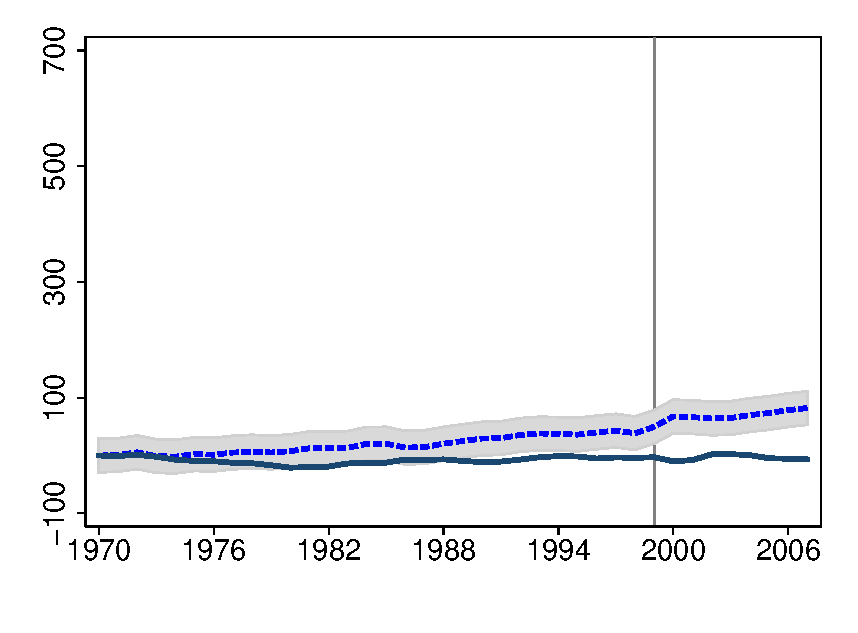
\includegraphics[width=8cm]{Composition/SCM_csh_nx_3_Annual.eps}}
    \annote{The plots depict, for each GDP component, the deviation in percent from the value of 1970. The blue dashed lines represents the synthetic Austria computed in section \ref{S_Doppelganger}. The full black lines stand for the actual Belgian series. The shaded area corresponds to two standard deviations of the difference between the treated country and the doppelganger prior to the euro accession. }
\end{figure}

\begin{figure}[h!]
    \centering
    \caption{\label{F_Components_FIN} Components of Finland's GDP}
    \subfigure[Private Consumption]{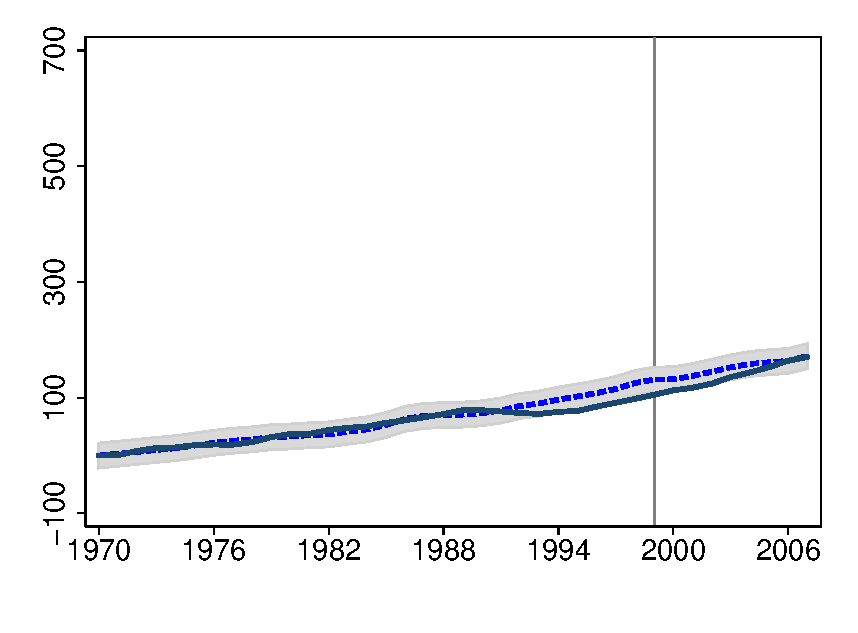
\includegraphics[width=8cm]{Composition/SCM_csh_c_7_Annual.eps}}
    \subfigure[Government Consumption]{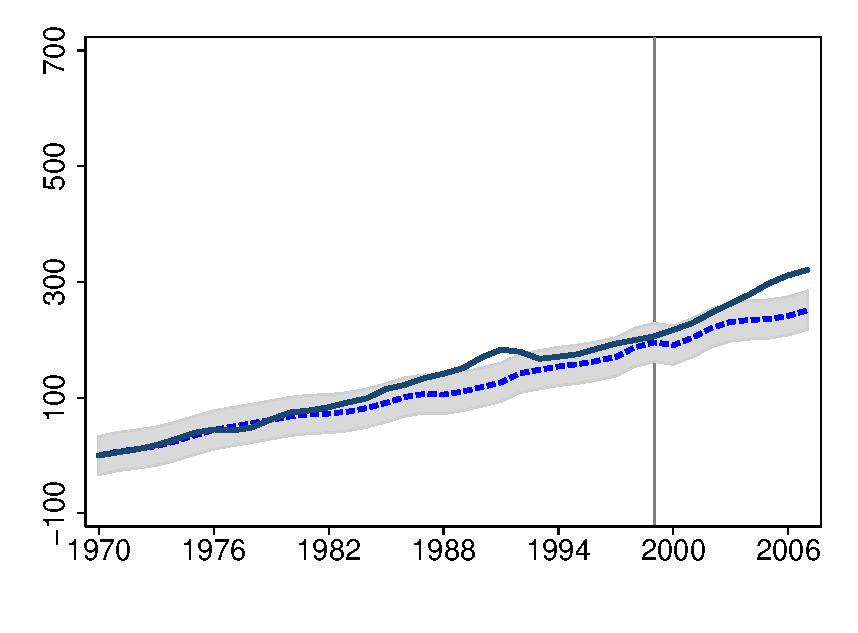
\includegraphics[width=8cm]{Composition/SCM_csh_g_7_Annual.eps}}
    \subfigure[Investment]{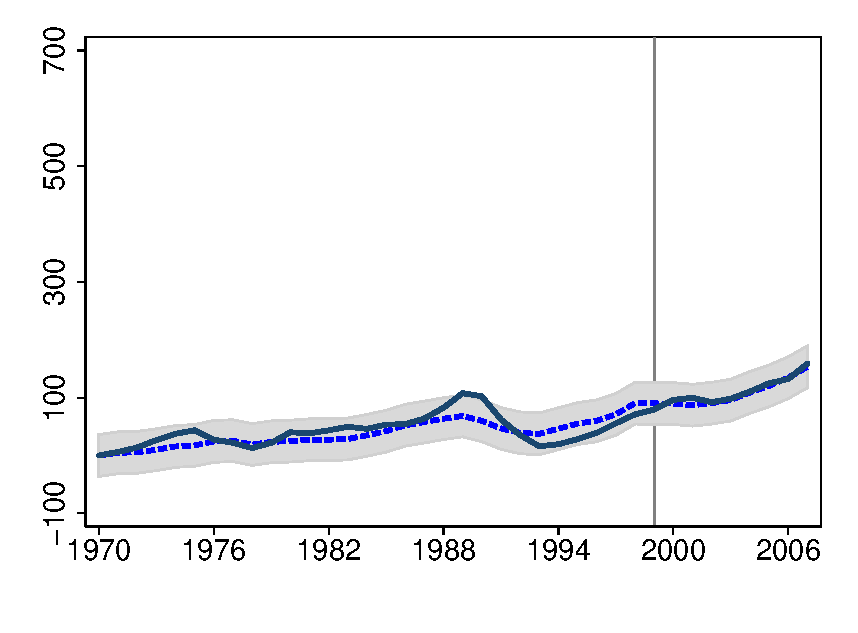
\includegraphics[width=8cm]{Composition/SCM_csh_i_7_Annual.eps}}
    \subfigure[Exports]{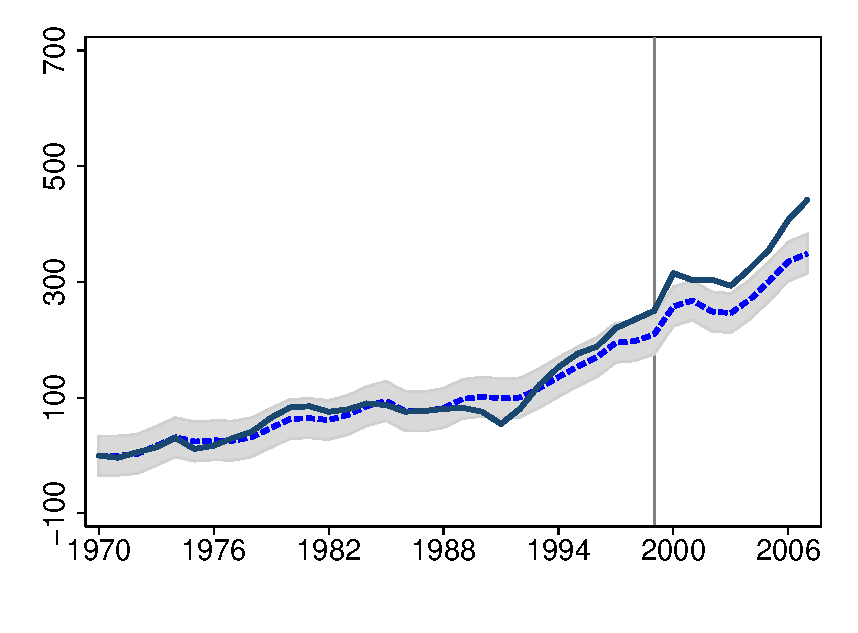
\includegraphics[width=8cm]{Composition/SCM_csh_x_7_Annual.eps}}
    \subfigure[Imports]{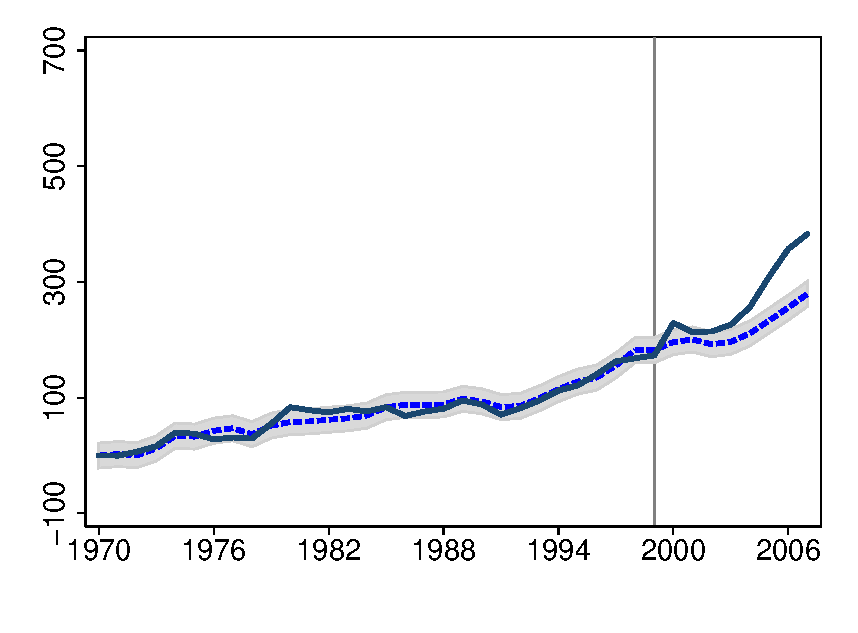
\includegraphics[width=8cm]{Composition/SCM_csh_m_7_Annual.eps}}
    \subfigure[Net Exports]{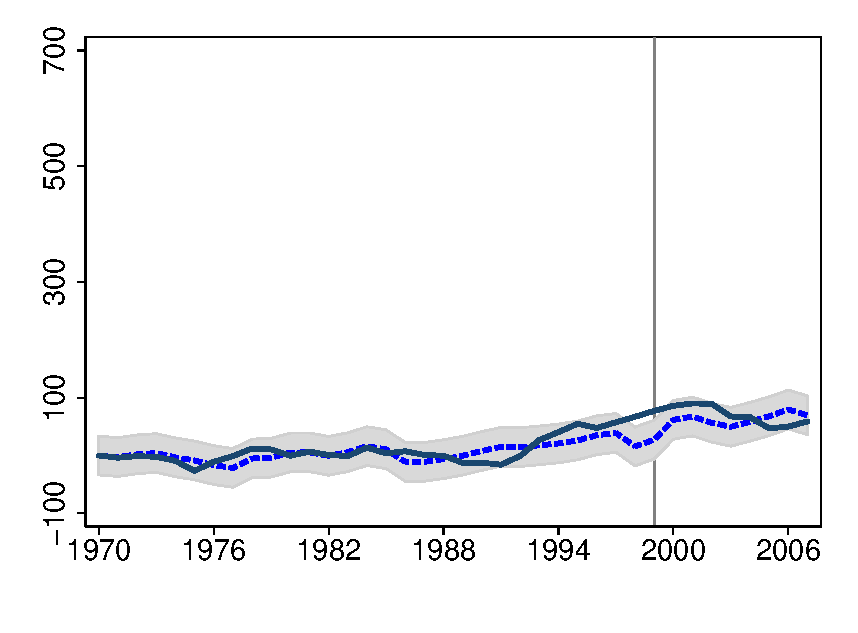
\includegraphics[width=8cm]{Composition/SCM_csh_nx_7_Annual.eps}}
    \annote{The plots depict, for each GDP component, the deviation in percent from the value of 1970. The blue dashed lines represents the synthetic Belgium computed in section \ref{S_Doppelganger}. The full black lines stand for the actual Finnish series. The shaded area corresponds to two standard deviations of the difference between the treated country and the doppelganger prior to the euro accession. }
\end{figure}

\begin{figure}[h!]
    \centering
    \caption{\label{F_Components_FRA} Components of France's GDP}
    \subfigure[Private Consumption]{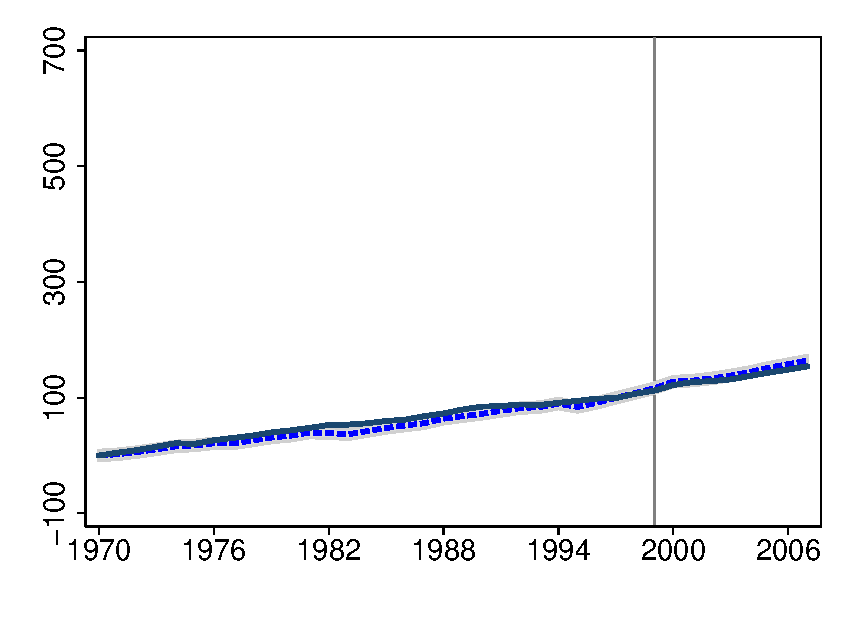
\includegraphics[width=8cm]{Composition/SCM_csh_c_8_Annual.eps}}
    \subfigure[Government Consumption]{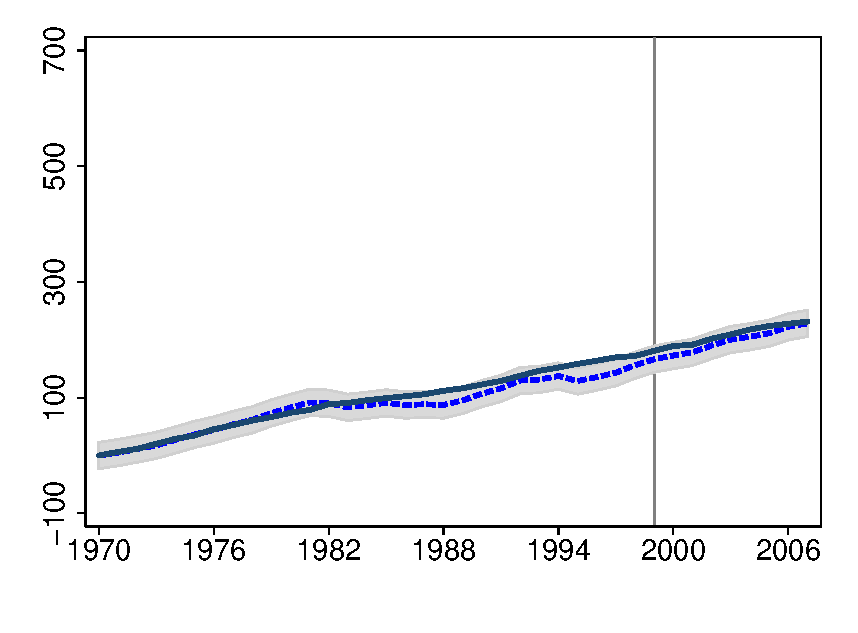
\includegraphics[width=8cm]{Composition/SCM_csh_g_8_Annual.eps}}
    \subfigure[Investment]{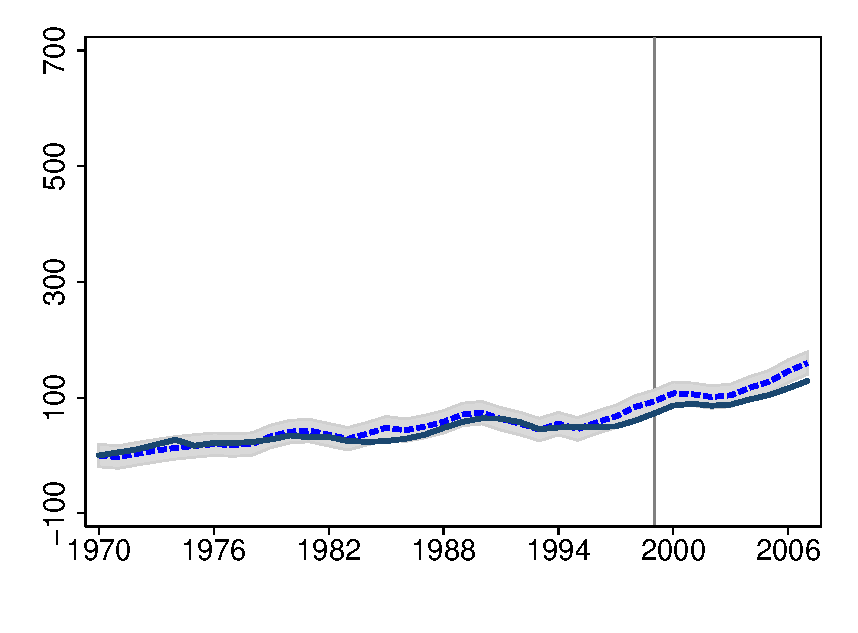
\includegraphics[width=8cm]{Composition/SCM_csh_i_8_Annual.eps}}
    \subfigure[Exports]{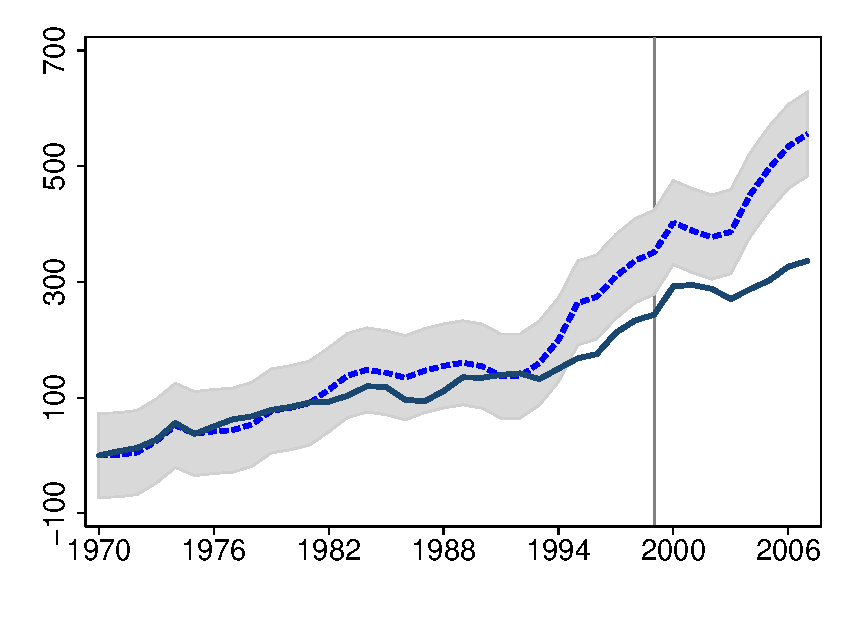
\includegraphics[width=8cm]{Composition/SCM_csh_x_8_Annual.eps}}
    \subfigure[Imports]{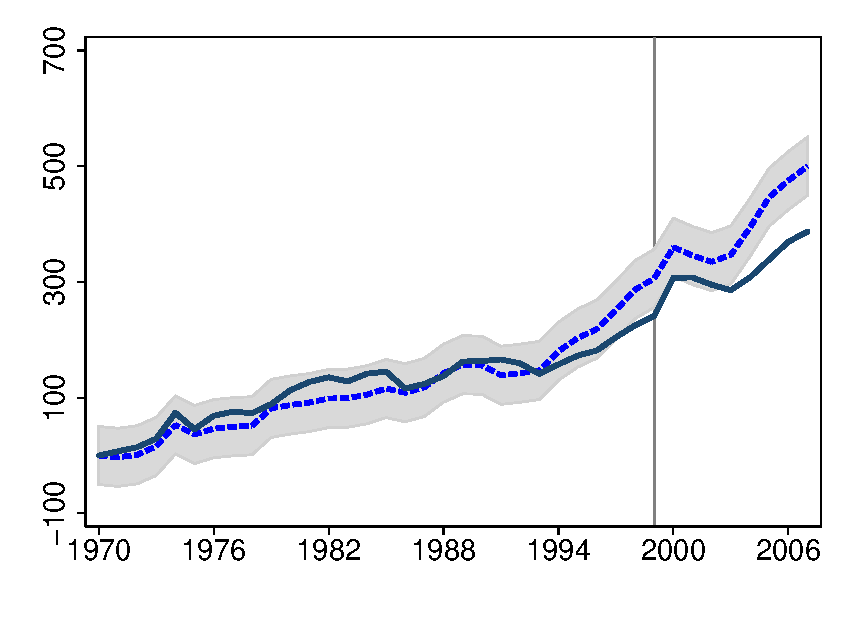
\includegraphics[width=8cm]{Composition/SCM_csh_m_8_Annual.eps}}
    \subfigure[Net Exports]{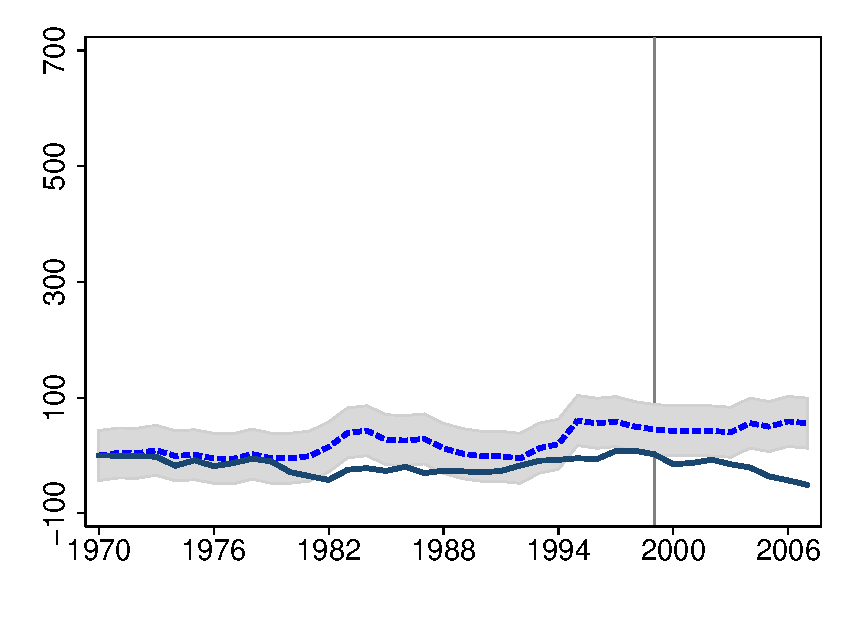
\includegraphics[width=8cm]{Composition/SCM_csh_nx_8_Annual.eps}}
    \annote{The plots depict, for each GDP component, the deviation in percent from the value of 1970. The blue dashed lines represents the synthetic France computed in section \ref{S_Doppelganger}. The full black lines stand for the actual French series. The shaded area corresponds to two standard deviations of the difference between the treated country and the doppelganger prior to the euro accession. }
\end{figure}

\begin{figure}[h!]
    \centering
    \caption{\label{F_Components_DEU} Components of Germany's GDP}
    \subfigure[Private Consumption]{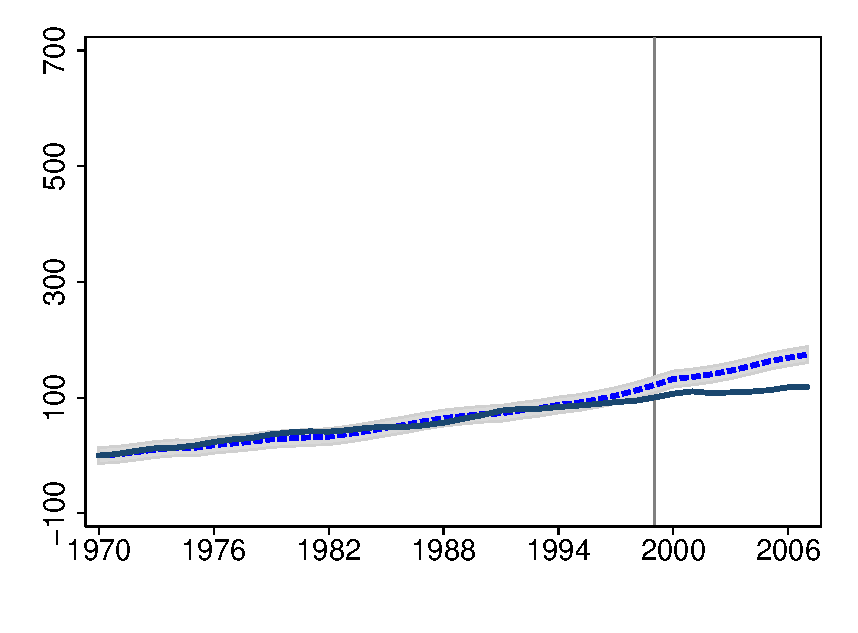
\includegraphics[width=8cm]{Composition/SCM_csh_c_9_Annual.eps}}
    \subfigure[Government Consumption]{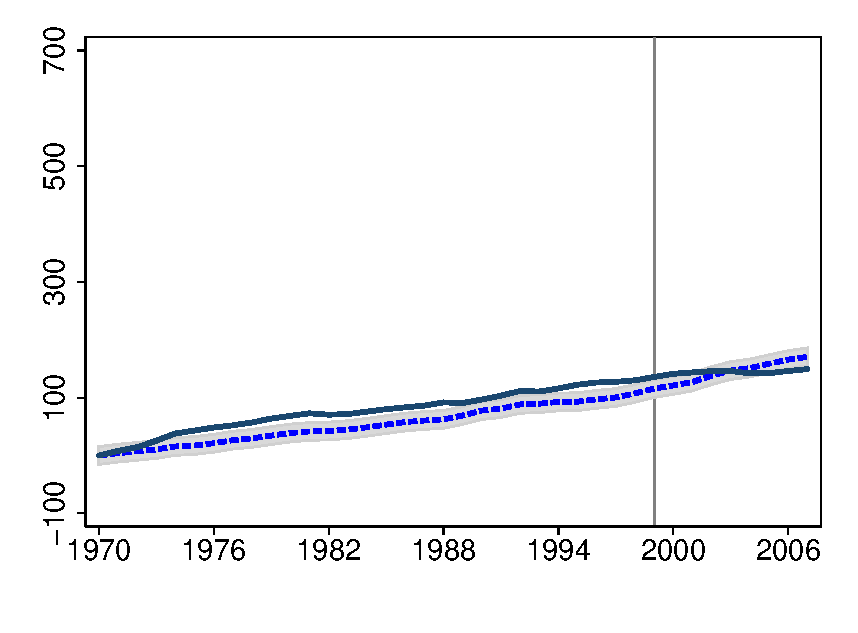
\includegraphics[width=8cm]{Composition/SCM_csh_g_9_Annual.eps}}
    \subfigure[Investment]{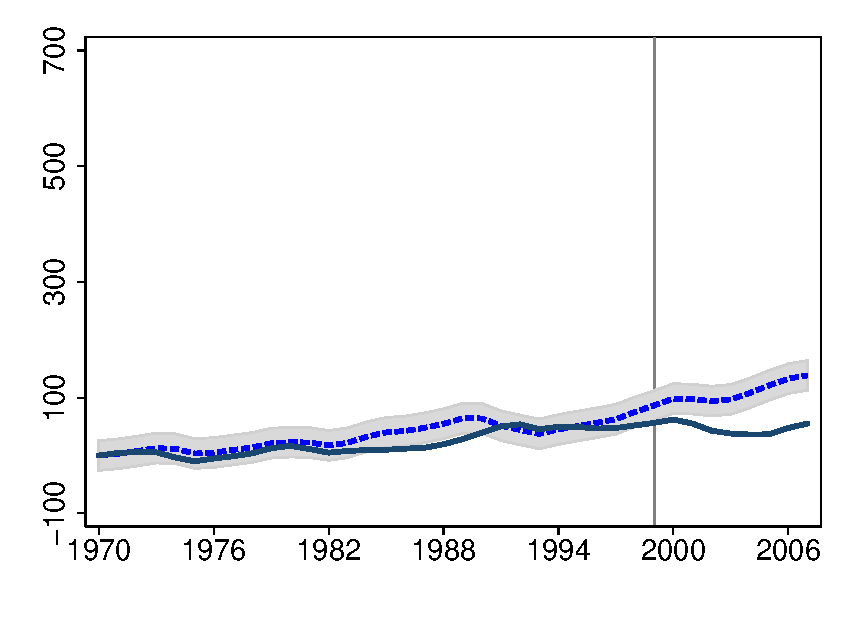
\includegraphics[width=8cm]{Composition/SCM_csh_i_9_Annual.eps}}
    \subfigure[Exports]{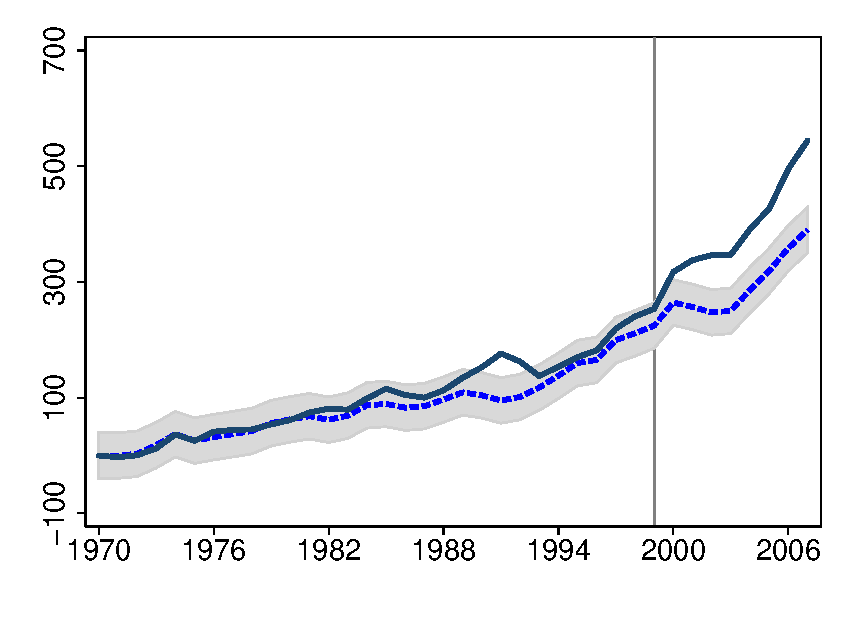
\includegraphics[width=8cm]{Composition/SCM_csh_x_9_Annual.eps}}
    \subfigure[Imports]{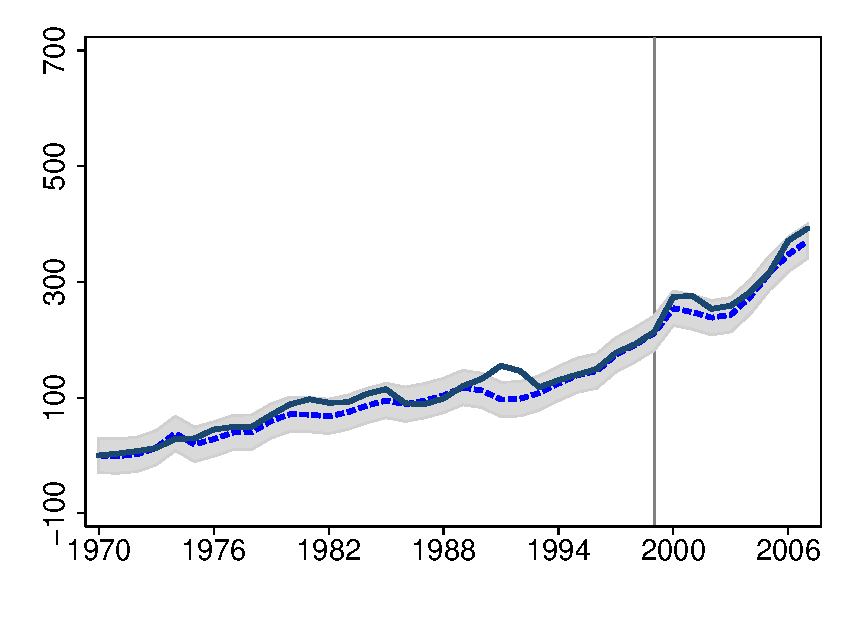
\includegraphics[width=8cm]{Composition/SCM_csh_m_9_Annual.eps}}
    \subfigure[Net Exports]{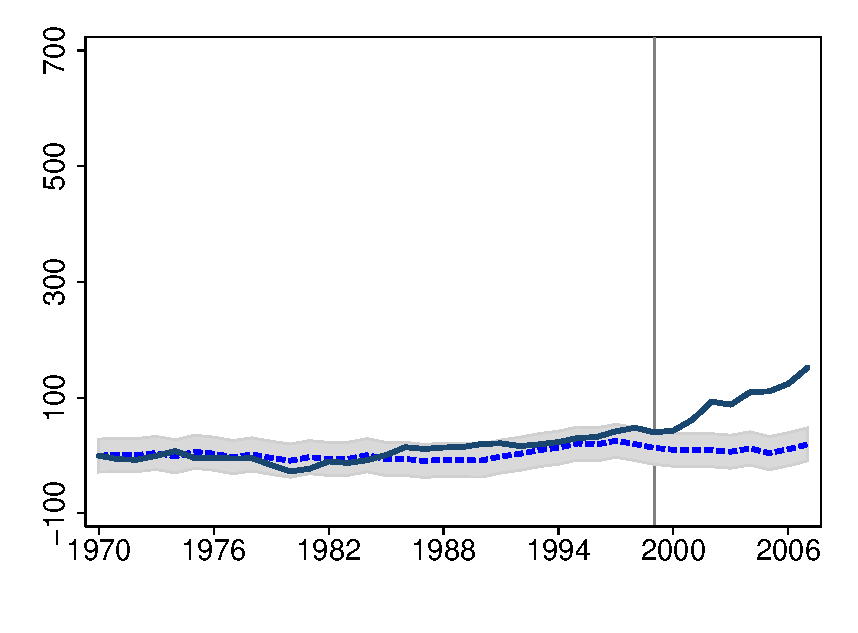
\includegraphics[width=8cm]{Composition/SCM_csh_nx_9_Annual.eps}}
    \annote{The plots depict, for each GDP component, the deviation in percent from the value of 1970. The blue dashed lines represents the synthetic Germany computed in section \ref{S_Doppelganger}. The full black lines stand for the actual German series. The shaded area corresponds to two standard deviations of the difference between the treated country and the doppelganger prior to the euro accession. }
\end{figure}

\begin{figure}[h!]
    \centering
    \caption{\label{F_Components_GRC} Components of Greece's GDP}
    \subfigure[Private Consumption]{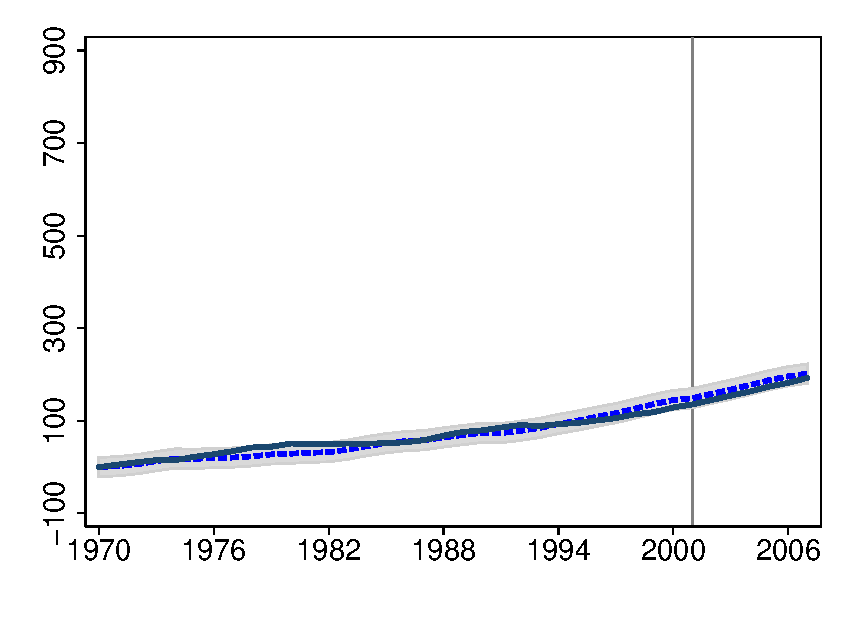
\includegraphics[width=8cm]{Composition/SCM_csh_c_10_Annual.eps}}
    \subfigure[Government Consumption]{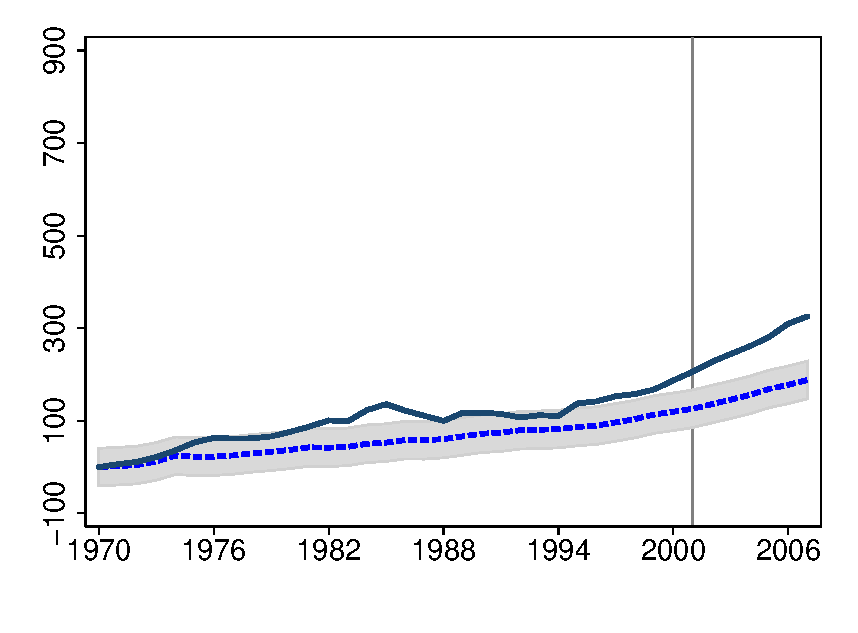
\includegraphics[width=8cm]{Composition/SCM_csh_g_10_Annual.eps}}
    \subfigure[Investment]{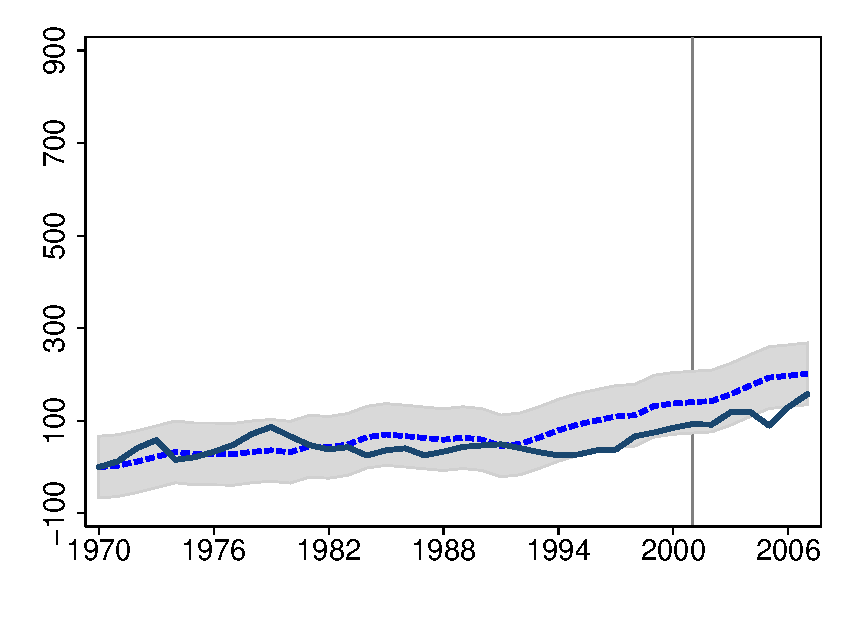
\includegraphics[width=8cm]{Composition/SCM_csh_i_10_Annual.eps}}
    \subfigure[Exports]{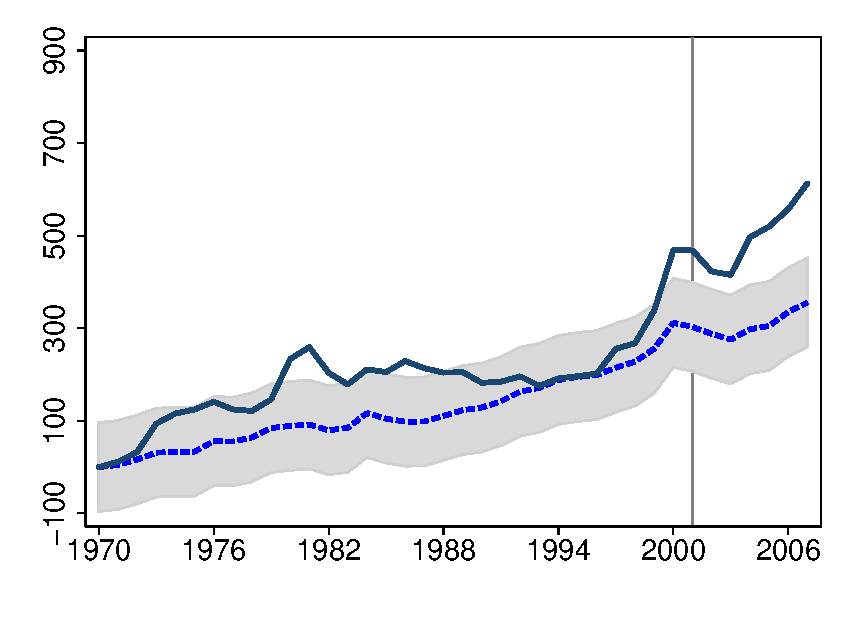
\includegraphics[width=8cm]{Composition/SCM_csh_x_10_Annual.eps}}
    \subfigure[Imports]{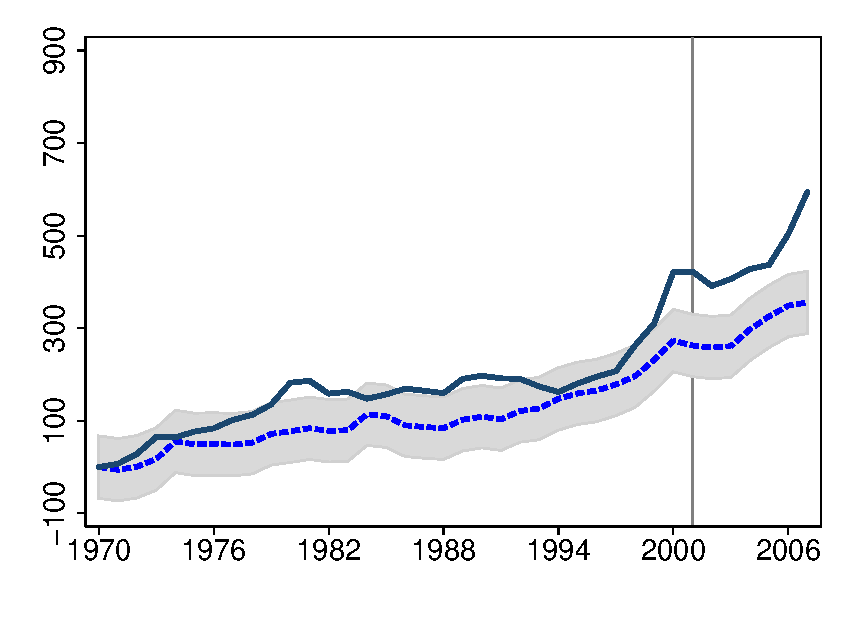
\includegraphics[width=8cm]{Composition/SCM_csh_m_10_Annual.eps}}
    \subfigure[Net Exports]{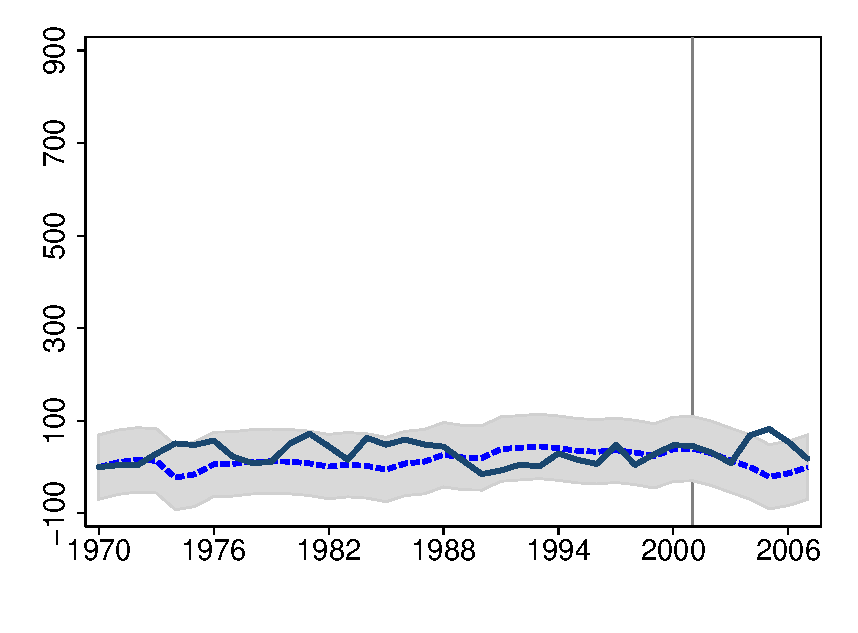
\includegraphics[width=8cm]{Composition/SCM_csh_nx_10_Annual.eps}}
    \annote{The plots depict, for each GDP component, the deviation in percent from the value of 1970. The blue dashed lines represents the synthetic Greece computed in section \ref{S_Doppelganger}. The full black lines stand for the actual Greek series. The shaded area corresponds to two standard deviations of the difference between the treated country and the doppelganger prior to the euro accession. }
\end{figure}

\begin{figure}[h!]
    \centering
    \caption{\label{F_Components_IRL} Components of Ireland's GDP}
    \subfigure[Private Consumption]{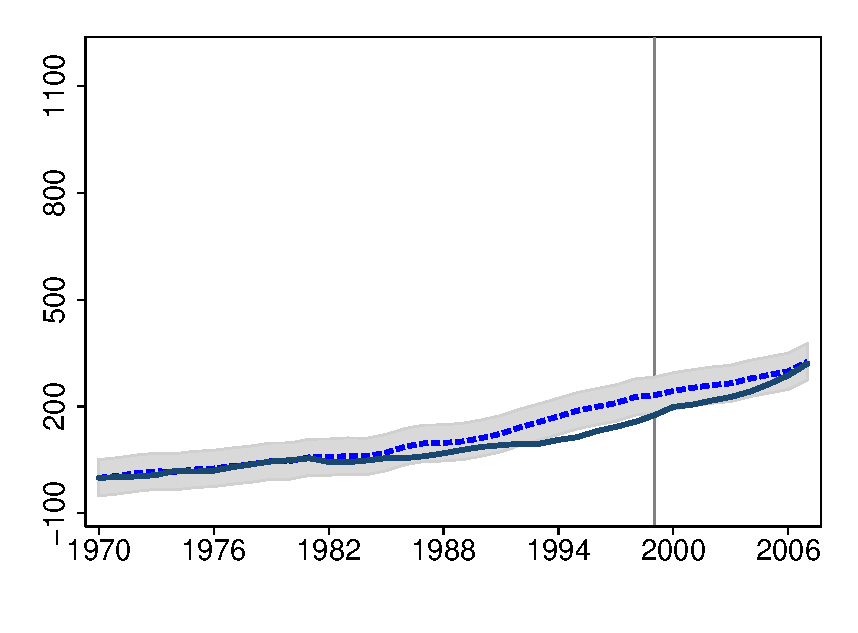
\includegraphics[width=8cm]{Composition/SCM_csh_c_12_Annual.eps}}
    \subfigure[Government Consumption]{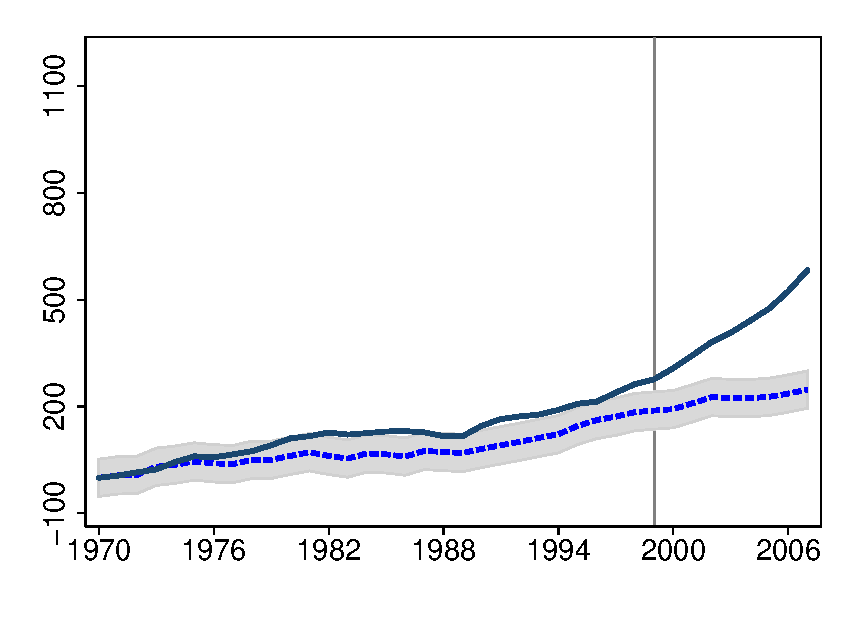
\includegraphics[width=8cm]{Composition/SCM_csh_g_12_Annual.eps}}
    \subfigure[Investment]{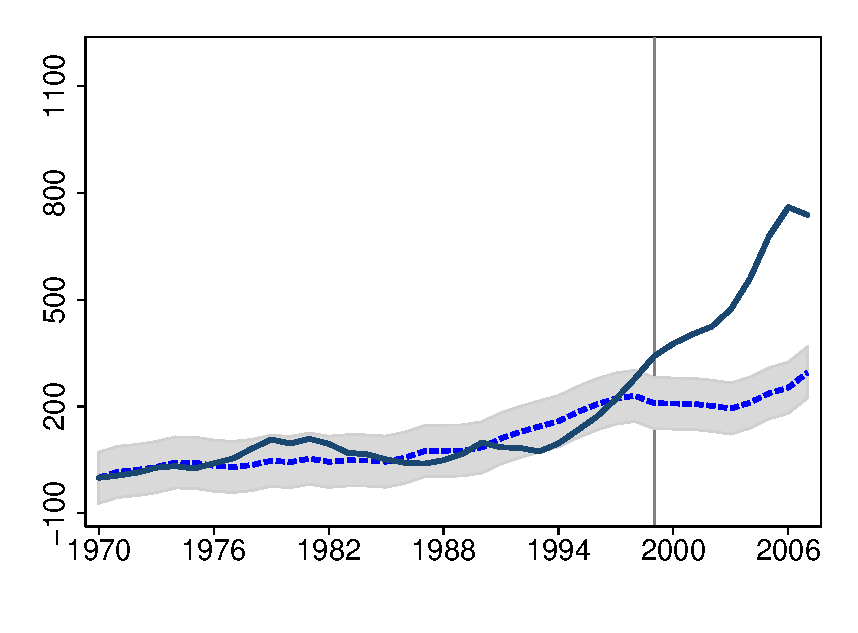
\includegraphics[width=8cm]{Composition/SCM_csh_i_12_Annual.eps}}
    \subfigure[Exports]{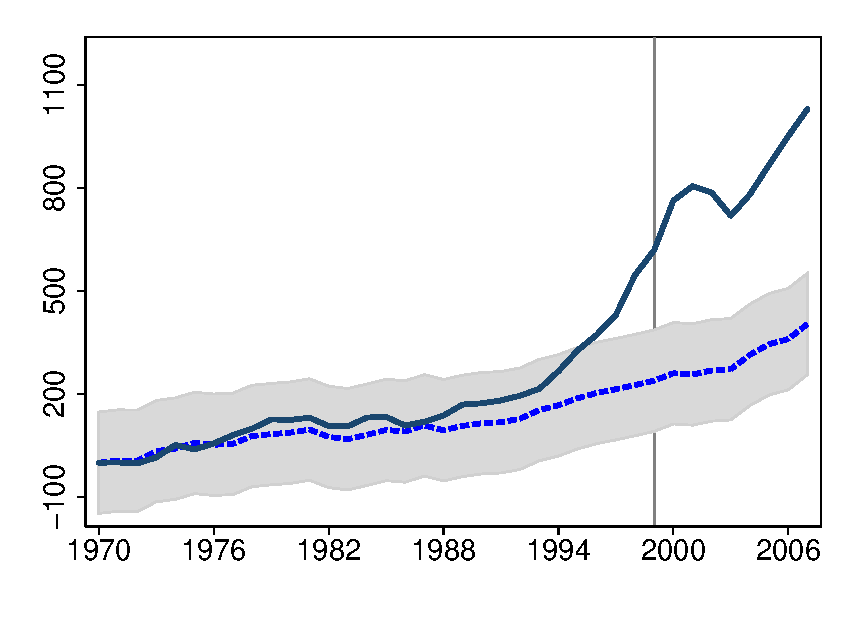
\includegraphics[width=8cm]{Composition/SCM_csh_m_12_Annual.eps}}
    \subfigure[Imports]{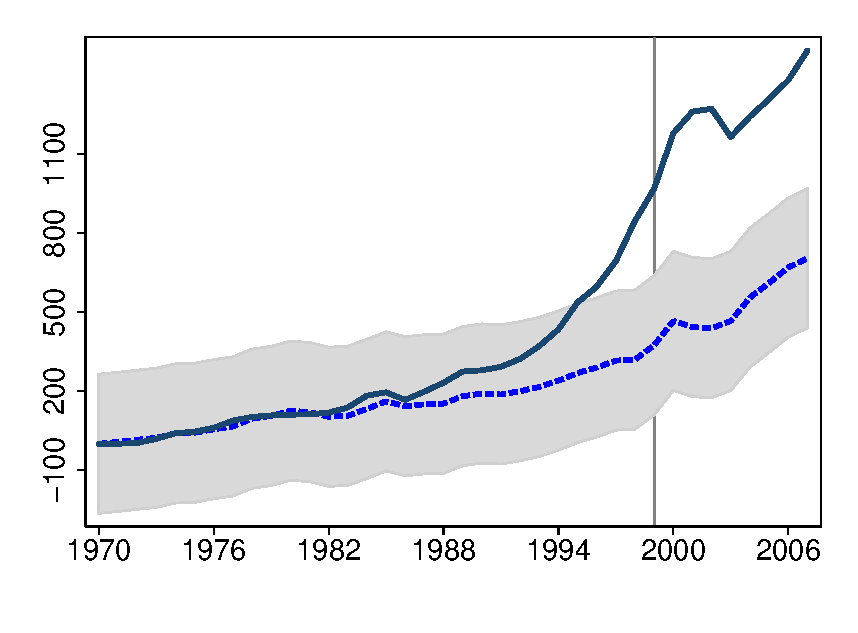
\includegraphics[width=8cm]{Composition/SCM_csh_x_12_Annual.eps}}
    \subfigure[Net Exports]{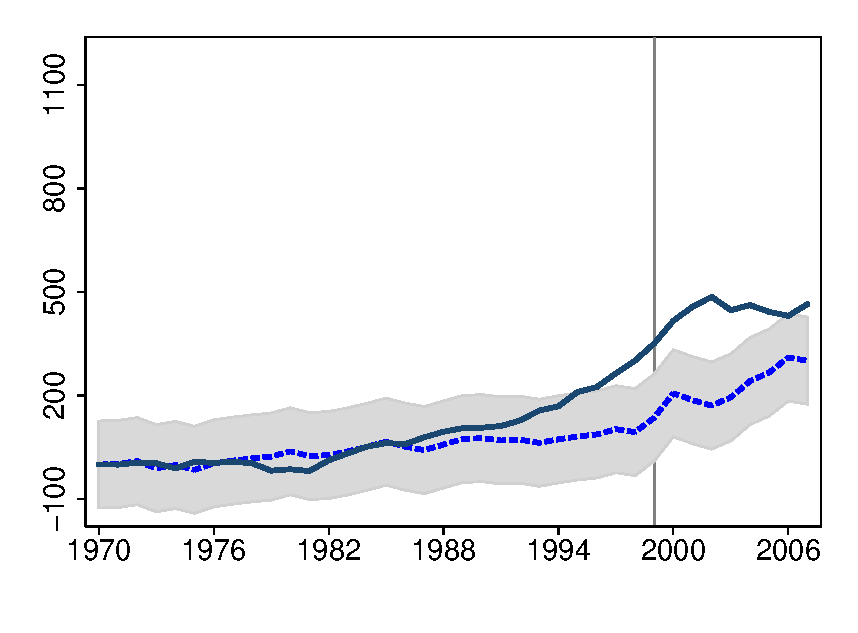
\includegraphics[width=8cm]{Composition/SCM_csh_nx_12_Annual.eps}}
    \annote{The plots depict, for each GDP component, the deviation in percent from the value of 1970. The blue dashed lines represents the synthetic Ireland computed in section \ref{S_Doppelganger}. The full black lines stand for the actual Irish series. The shaded area corresponds to two standard deviations of the difference between the treated country and the doppelganger prior to the euro accession. }
\end{figure}

\begin{figure}[h!]
    \centering
    \caption{\label{F_Components_ITA} Components of Italy's GDP}
    \subfigure[Private Consumption]{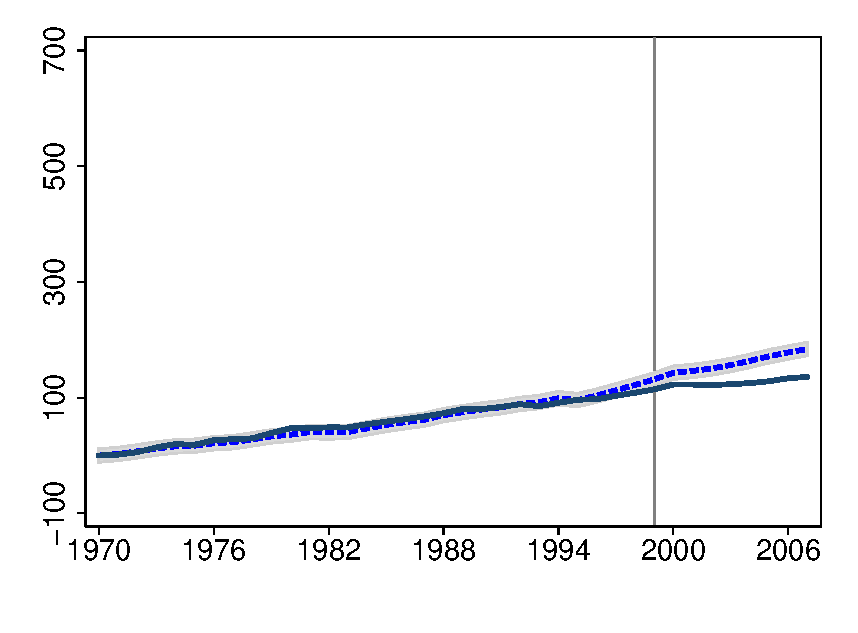
\includegraphics[width=8cm]{Composition/SCM_csh_c_14_Annual.eps}}
    \subfigure[Government Consumption]{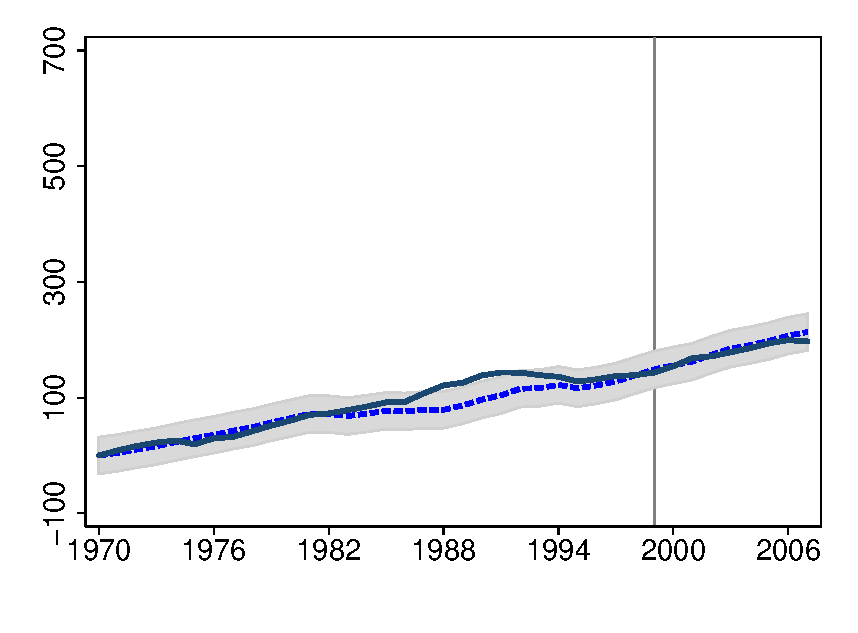
\includegraphics[width=8cm]{Composition/SCM_csh_g_14_Annual.eps}}
    \subfigure[Investment]{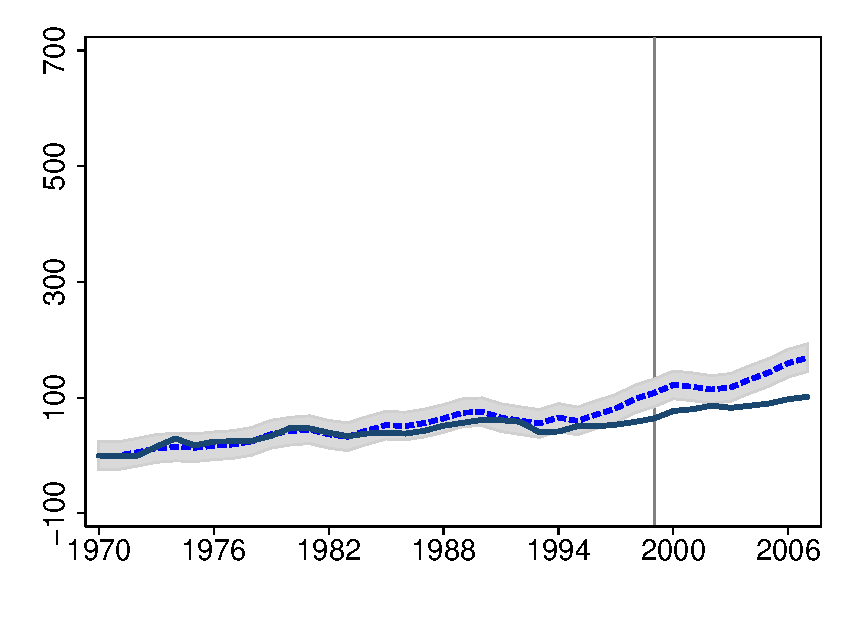
\includegraphics[width=8cm]{Composition/SCM_csh_i_14_Annual.eps}}
    \subfigure[Exports]{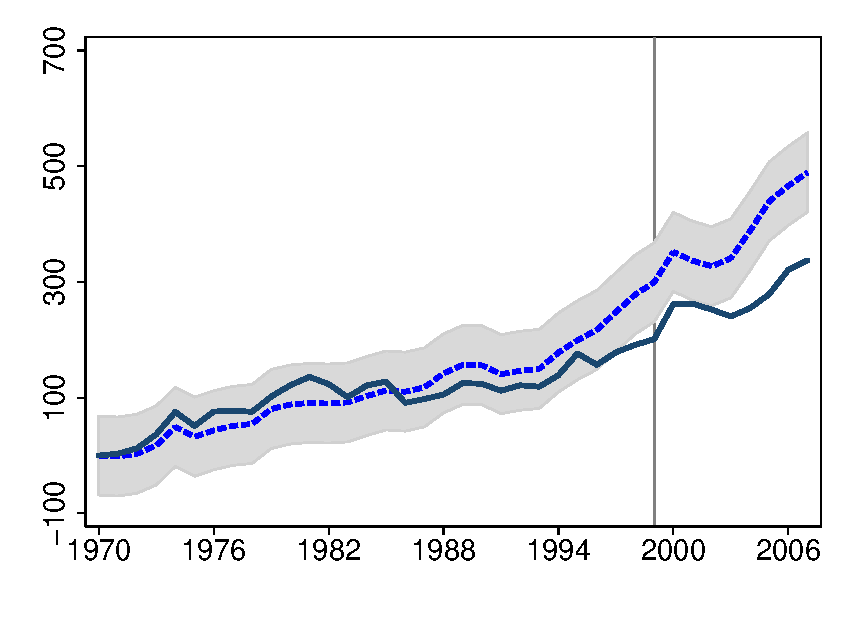
\includegraphics[width=8cm]{Composition/SCM_csh_m_14_Annual.eps}}
    \subfigure[Imports]{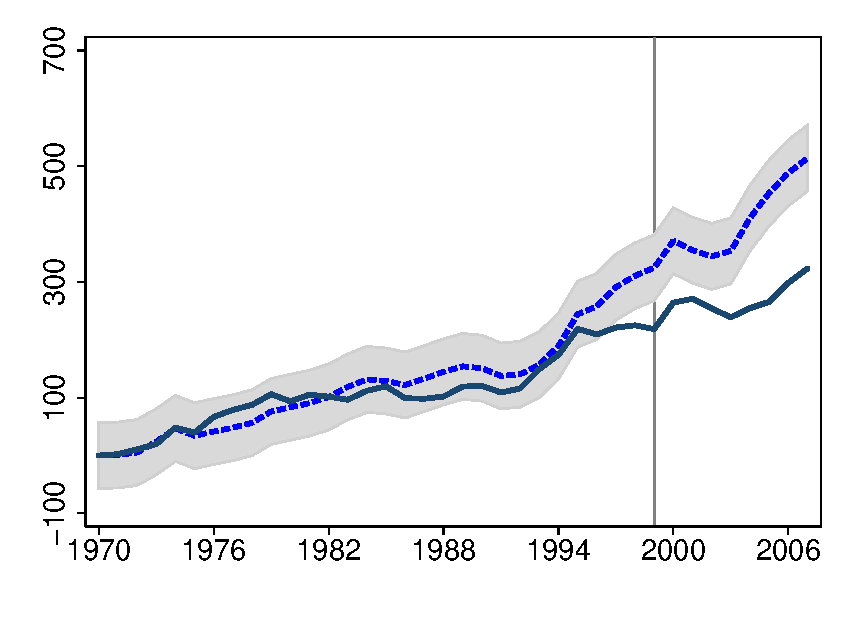
\includegraphics[width=8cm]{Composition/SCM_csh_x_14_Annual.eps}}
    \subfigure[Net Exports]{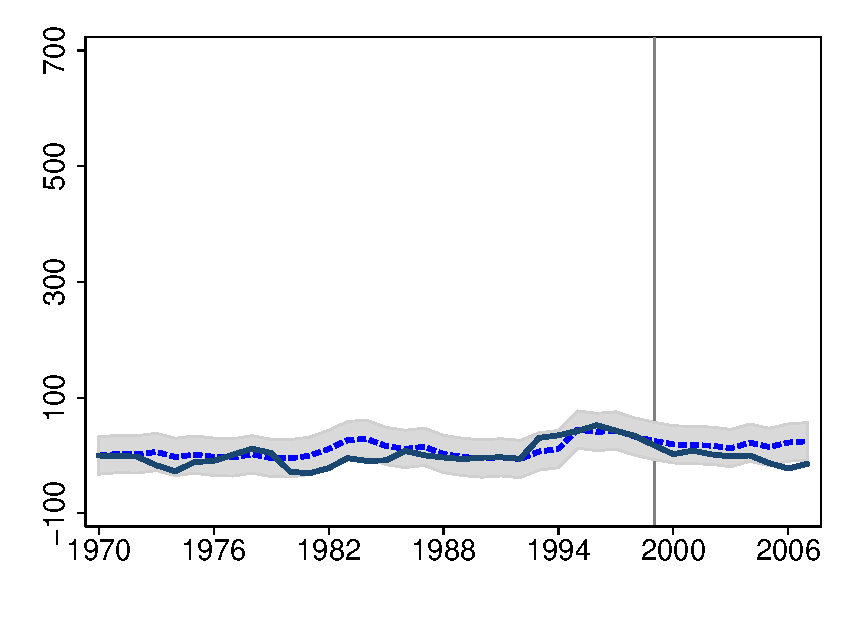
\includegraphics[width=8cm]{Composition/SCM_csh_nx_14_Annual.eps}}
    \annote{The plots depict, for each GDP component, the deviation in percent from the value of 1970. The blue dashed lines represents the synthetic Italy computed in section \ref{S_Doppelganger}. The full black lines stand for the actual Italian series. The shaded area corresponds to two standard deviations of the difference between the treated country and the doppelganger prior to the euro accession. }
\end{figure}

\begin{figure}[h!]
    \centering
    \caption{\label{F_Components_LUX} Components of Luxembourg's GDP}
    \subfigure[Private Consumption]{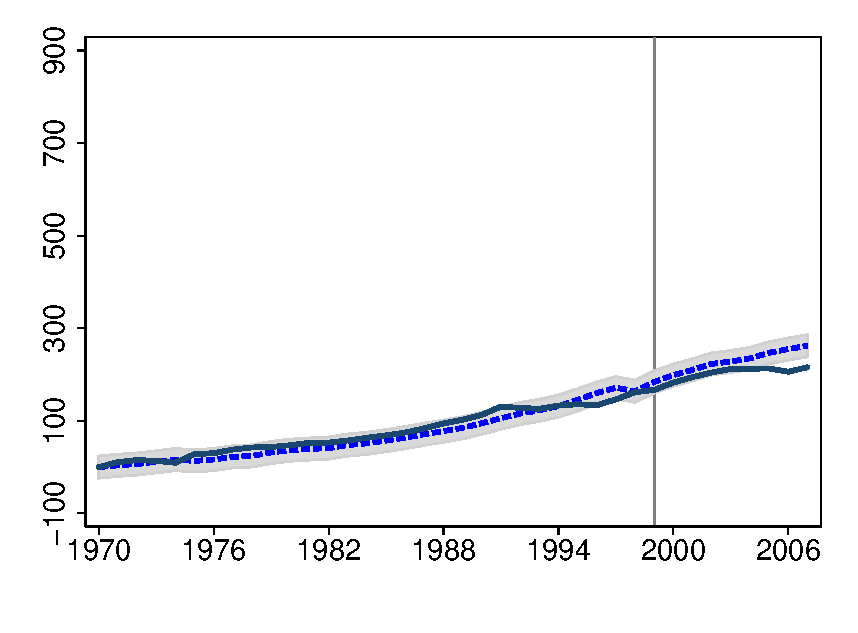
\includegraphics[width=8cm]{Composition/SCM_csh_c_16_Annual.eps}}
    \subfigure[Government Consumption]{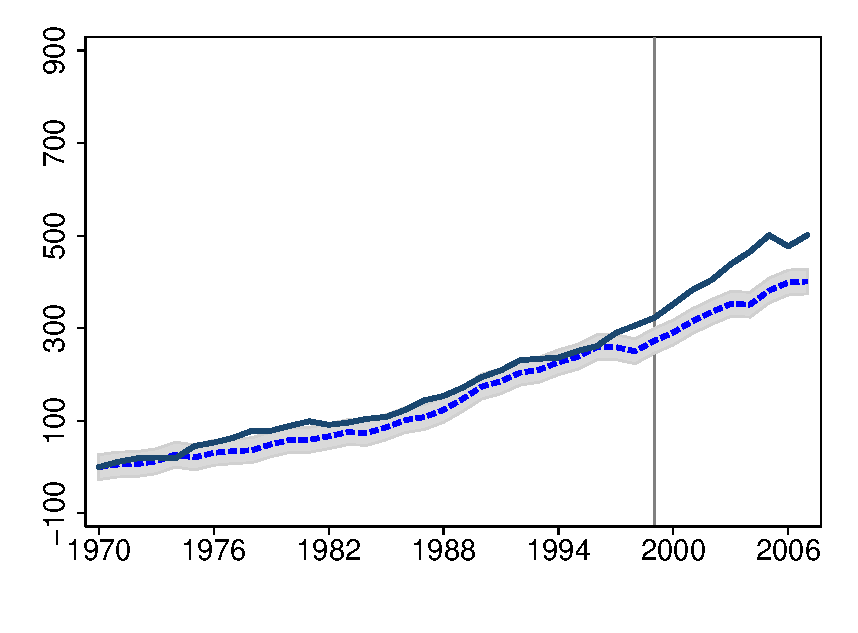
\includegraphics[width=8cm]{Composition/SCM_csh_g_16_Annual.eps}}
    \subfigure[Investment]{\includegraphics[width=8cm]{Composition/SCM_csh_i_16_Annual.eps}}
    \subfigure[Exports]{\includegraphics[width=8cm]{Composition/SCM_csh_x_16_Annual.eps}}
    \subfigure[Imports]{\includegraphics[width=8cm]{Composition/SCM_csh_m_16_Annual.eps}}
    \subfigure[Net Exports]{\includegraphics[width=8cm]{Composition/SCM_csh_nx_16_Annual.eps}}
    \annote{The plots depict, for each GDP component, the deviation in percent from the value of 1970. The blue dashed lines represents the synthetic Luxembourg computed in section \ref{S_Doppelganger}. The full black lines stand for the actual Luxembourg's series. The shaded area corresponds to two standard deviations of the difference between the treated country and the doppelganger prior to the euro accession. }
\end{figure}

\begin{figure}[h!]
    \centering
    \caption{\label{F_Components_NLD} Components of The Netherlands's GDP}
    \subfigure[Private Consumption]{\includegraphics[width=8cm]{Composition/SCM_csh_c_18_Annual.eps}}
    \subfigure[Government Consumption]{\includegraphics[width=8cm]{Composition/SCM_csh_g_18_Annual.eps}}
    \subfigure[Investment]{\includegraphics[width=8cm]{Composition/SCM_csh_i_18_Annual.eps}}
    \subfigure[Exports]{\includegraphics[width=8cm]{Composition/SCM_csh_x_18_Annual.eps}}
    \subfigure[Imports]{\includegraphics[width=8cm]{Composition/SCM_csh_m_18_Annual.eps}}
    \subfigure[Net Exports]{\includegraphics[width=8cm]{Composition/SCM_csh_nx_18_Annual.eps}}
    \annote{The plots depict, for each GDP component, the deviation in percent from the value of 1970. The blue dashed lines represents the synthetic Netherlands computed in section \ref{S_Doppelganger}. The full black lines stand for the actual Dutch series. The shaded area corresponds to two standard deviations of the difference between the treated country and the doppelganger prior to the euro accession.}
\end{figure}

\begin{figure}[h!]
    \centering
    \caption{\label{F_Components_PRT} Components of Portugal's GDP}
    \subfigure[Private Consumption]{\includegraphics[width=8cm]{Composition/SCM_csh_c_21_Annual.eps}}
    \subfigure[Government Consumption]{\includegraphics[width=8cm]{Composition/SCM_csh_g_21_Annual.eps}}
    \subfigure[Investment]{\includegraphics[width=8cm]{Composition/SCM_csh_i_21_Annual.eps}}
    \subfigure[Exports]{\includegraphics[width=8cm]{Composition/SCM_csh_x_21_Annual.eps}}
    \subfigure[Imports]{\includegraphics[width=8cm]{Composition/SCM_csh_m_21_Annual.eps}}
    \subfigure[Net Exports]{\includegraphics[width=8cm]{Composition/SCM_csh_nx_21_Annual.eps}}
    \annote{The plots depict, for each GDP component, the deviation in percent from the value of 1970. The blue dashed lines represents the synthetic Portugal computed in section \ref{S_Doppelganger}. The full black lines stand for the actual Portuguese series.  The shaded area corresponds to two standard deviations of the difference between the treated country and the doppelganger prior to the euro accession.}
\end{figure}

\begin{figure}[h!]
    \centering
    \caption{\label{F_Components_ESP} Components of Spain's GDP}
    \subfigure[Private Consumption]{\includegraphics[width=8cm]{Composition/SCM_csh_c_22_Annual.eps}}
    \subfigure[Government Consumption]{\includegraphics[width=8cm]{Composition/SCM_csh_g_22_Annual.eps}}
    \subfigure[Investment]{\includegraphics[width=8cm]{Composition/SCM_csh_i_22_Annual.eps}}
    \subfigure[Exports]{\includegraphics[width=8cm]{Composition/SCM_csh_x_22_Annual.eps}}
    \subfigure[Imports]{\includegraphics[width=8cm]{Composition/SCM_csh_m_22_Annual.eps}}
    \subfigure[Net Exports]{\includegraphics[width=8cm]{Composition/SCM_csh_nx_22_Annual.eps}}
    \annote{The plots depict, for each GDP component, the deviation in percent from the value of 1970. The blue dashed lines represents the synthetic Spain computed in section \ref{S_Doppelganger}. The full black lines stand for the actual Spanish series. The shaded area corresponds to two standard deviations of the difference between the treated country and the doppelganger prior to the euro accession.}
\end{figure}

\end{document}